\documentclass[11pt]{article}
\usepackage{graphicx, subcaption}
\usepackage[top=1in, bottom=1in, left=1in, right=1in]{geometry}
\graphicspath{ {./figs/} }
\pagestyle{plain}
\def\changemargin#1#2{\list{}{\rightmargin#2\leftmargin#1}\item[]}
\let\endchangemargin=\endlist 
\begin{document}
\title{\vspace{-5mm}Edge-Conservative Reconnecting Model Timescales}
\author{Alexander Holiday}
\maketitle

We are attempting to numerically locate the separate timescales present in the edge conservative reconnecting model. In \cite{Rath2012}, you show that the dynamics create two separate timescales, one of order $n^{2}$, the other $n^{3}$. Seeing these computationally has proven difficult. Figs. \ref{fig:100s3} to \ref{fig:1000lv} show the evolution of the degree distribution from our numerical implementation of the model at system sizes of $n=100, 500$ and $1000$ and $\kappa = 0.5$. They are arranged as follows: for each system size, there are six figures, three of the $n^{2}$ timescale, three of the $n^{3}$. The first of the three is a direct 3D plot of the distribution vs. time. The second is a projection along the ``time'' axis, with data from earlier steps plotted with a higher transparency. The third is a projection along the ``percentile'' axis. The color in the plots illustrates the shape of the distribution at each step. Specifically, it tracks the evolution of the different percentiles. Thus, the maximum degree is colored dark red, the median is colored pale green, and the minimum dark blue. We might expect that the bands of color evolve slowly over the $n^{3}$ scale towards a steady state. Instead, it appears that the system quickly reaches its final state, approximately within $n^{3}$ steps, at which point significant evolution ceases (minor variations would be expected from the stochastic nature of the dynamics). I've considered two possible explanations for this difficulty, and I'm wondering if you have any insights yourself. The first is that the timescales are not purely $n^{2}$ and $n^{3}$, but, as you show, are $\frac{\rho(W)}{2} n^{2}$ and $\rho(W) n^{3}$. Unfortunately, the calculation of $\rho(W)$ does not appear straightforward, and thus it is difficult to test this hypothesis. Second, these results are proven in the limit of $n \rightarrow \infty$, and our finite system may not exhibit similar properties.
\bibliographystyle{abbrv}
\bibliography{$HOME/Documents/bibTex/library}

\begin{changemargin}{0.0cm}{0.0cm}
\centering

\centering
\begin{figure}[h!]
  \vspace{-30mm}
  \begin{subfigure}{0.5\textwidth}
    \includegraphics[height=60mm]{n_500_n3_3d_v2}
    \caption{$n^{3}$ timescale}
    \label{fig:100s3}
  \end{subfigure}%
  \begin{subfigure}{0.5\textwidth}
    \includegraphics[height=60mm]{n_500_2n3_3d_v2}
    \caption{$n^{2}$ timescale}
    \label{fig:100s3}
  \end{subfigure}%
  \caption{Evolution of degrees. ($n=500$, $m=250000$)}
  \label{fig:n500_3d}
\end{figure}

\begin{figure}[h!]
  \vspace{-5mm}
  \centering
  \begin{subfigure}{0.5\textwidth}
    \centering
    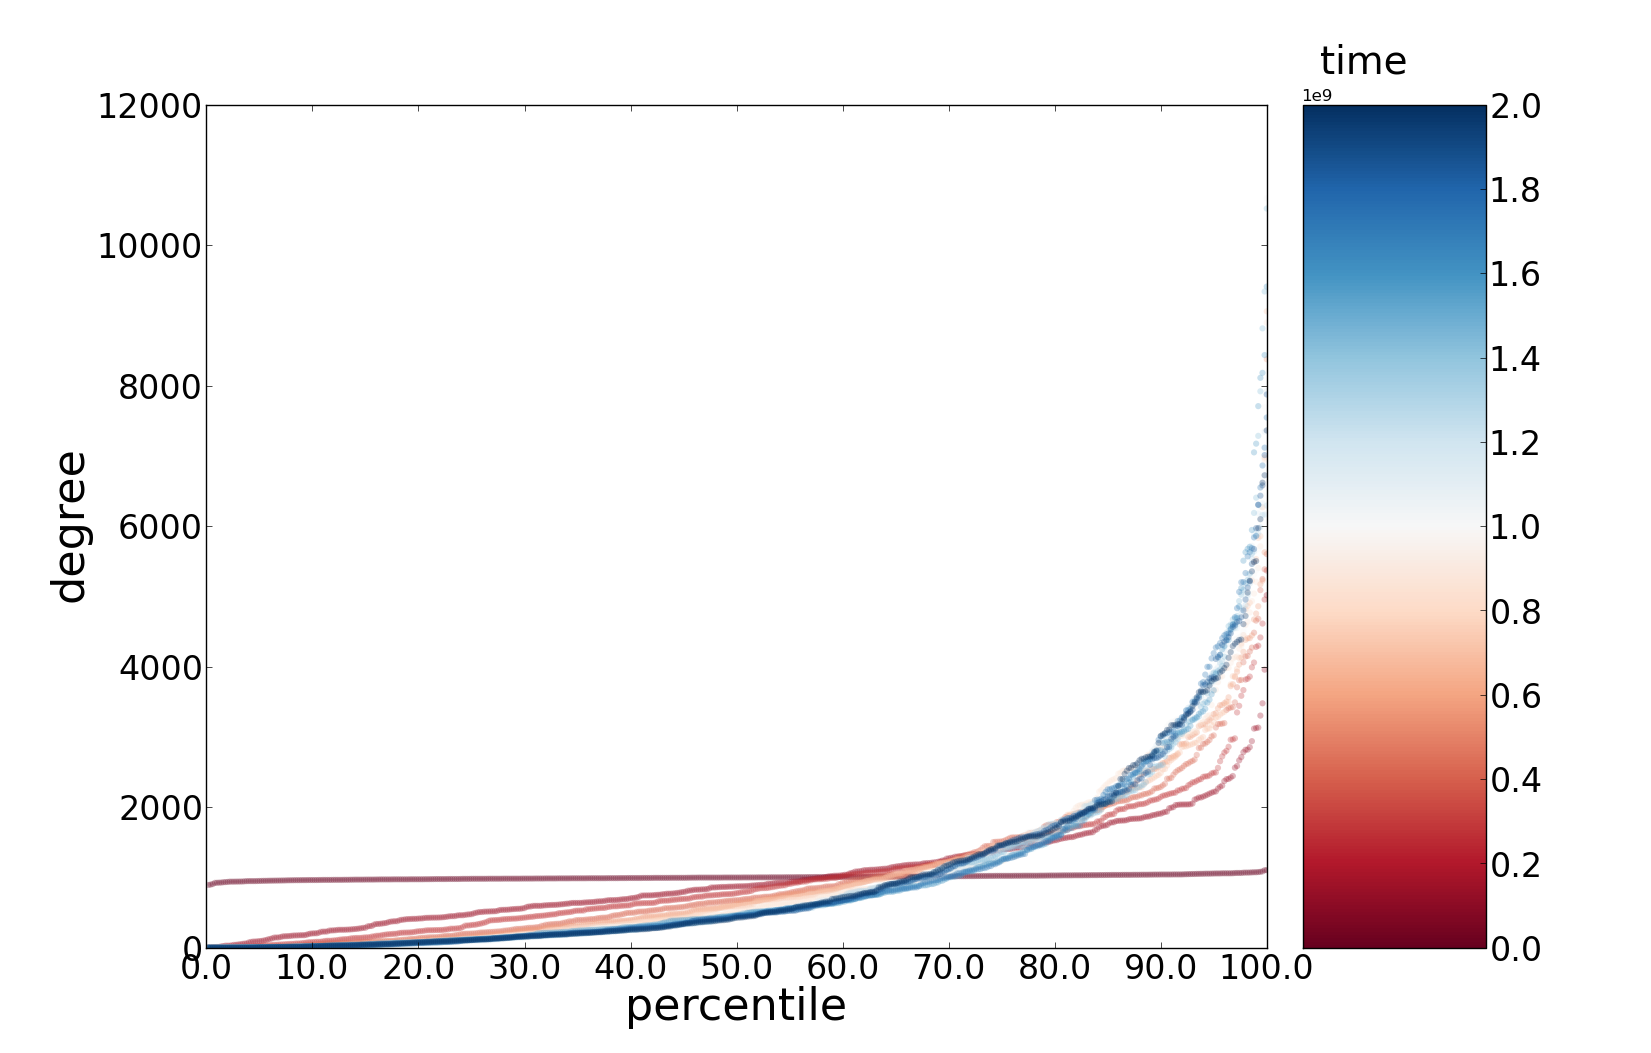
\includegraphics[height=50mm]{n_500_n3_deg_percentile}
    \caption{$n^{3}$ timescale}
    \label{fig:100s3}
  \end{subfigure}%
  \begin{subfigure}{0.5\textwidth}
    \centering
    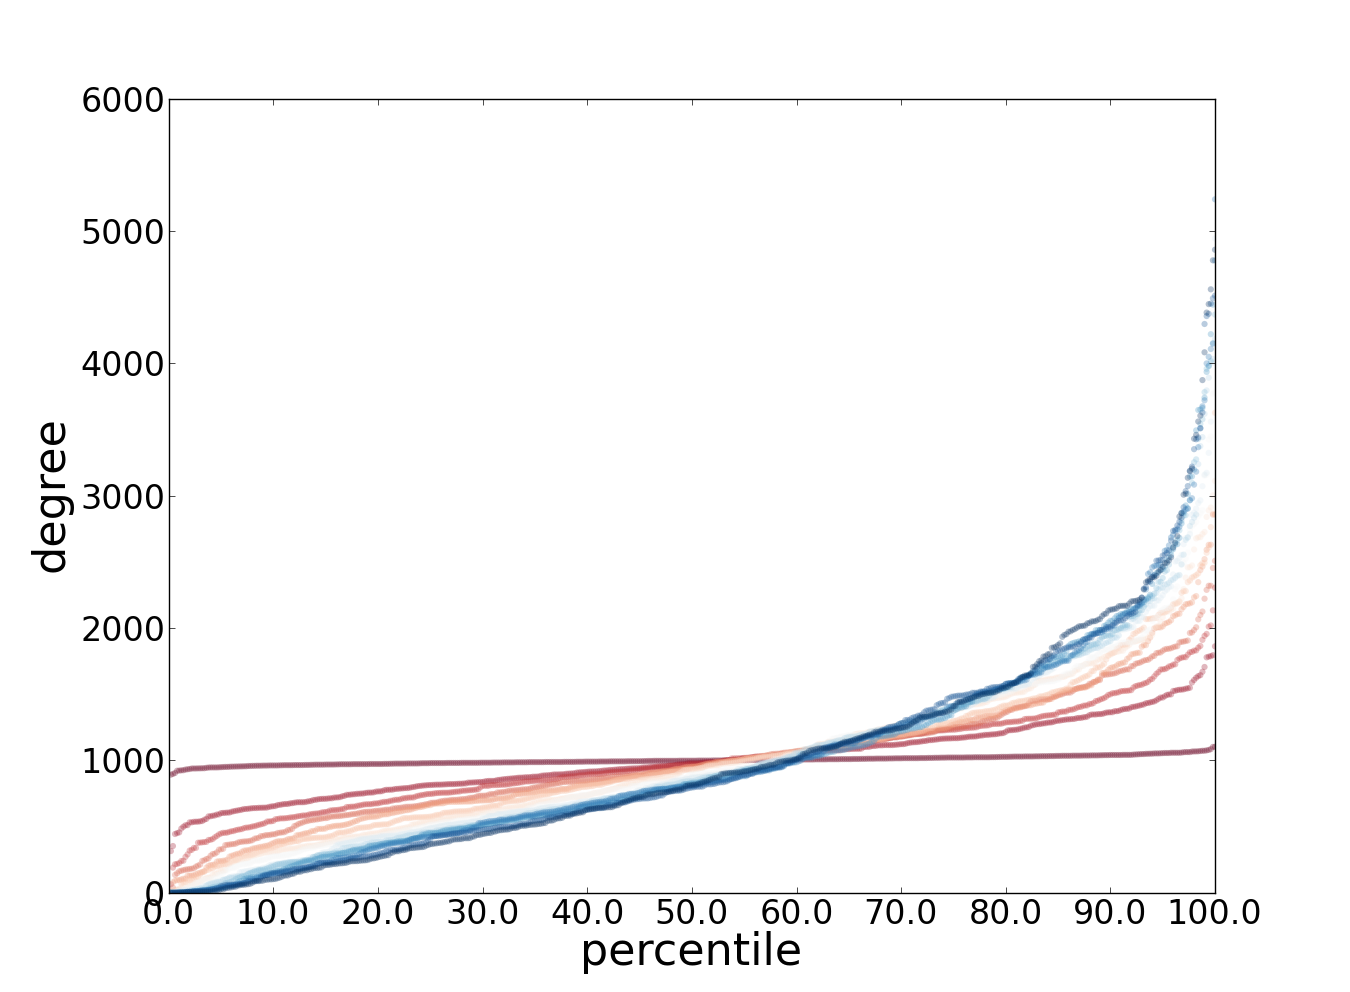
\includegraphics[height=50mm]{n_500_2n3_deg_percentile}
    \caption{$n^{2}$ timescale}
    \label{fig:100s3}
  \end{subfigure}%
  \caption{Evolution of degrees and percentiles, a projection of Fig. \ref{fig:n500_3d} along the time axis. ($n=500$, $m=250000$)}
\end{figure}

\begin{figure}[h!]
  \vspace{-5mm}
  \centering
  \begin{subfigure}{0.5\textwidth}
    \centering
    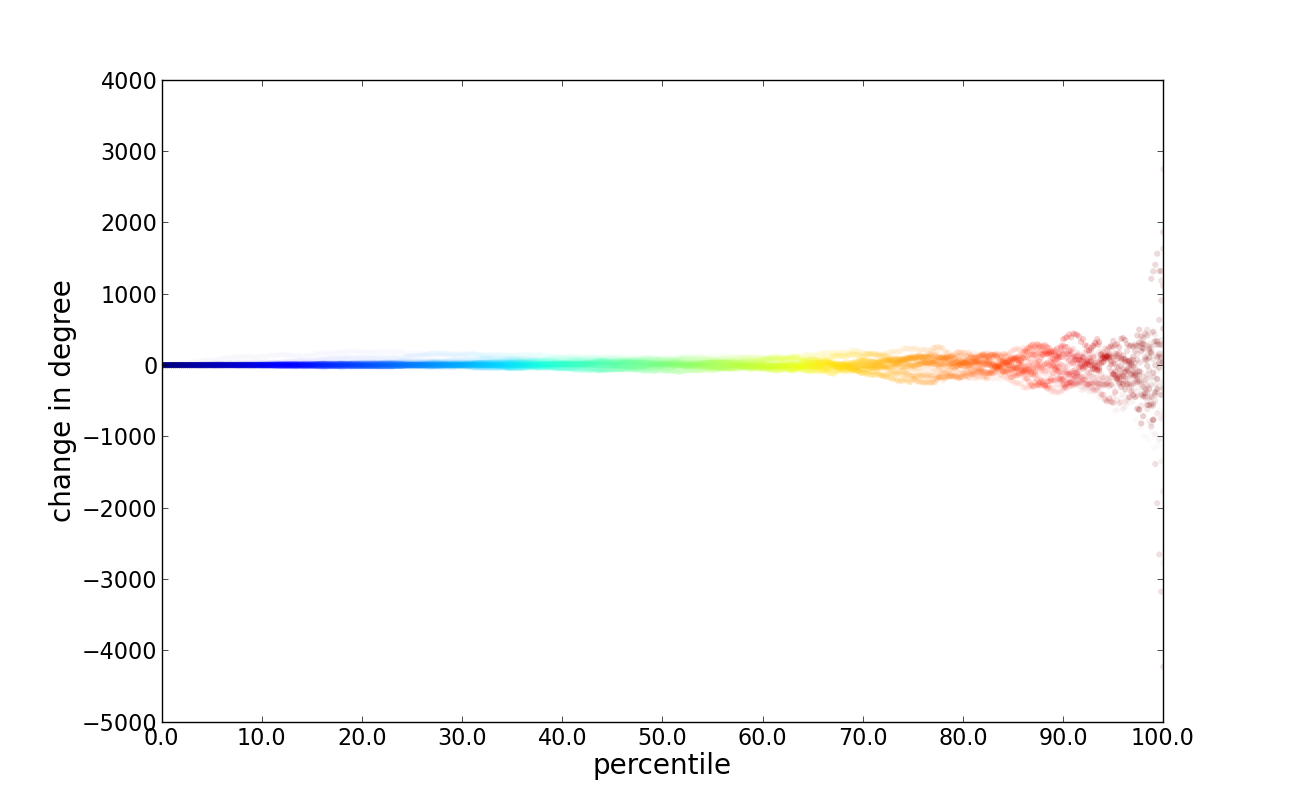
\includegraphics[height=60mm]{n_500_n3_degchange_percentile}
    \caption{$n^{3}$ timescale}
    \label{fig:100s3}
  \end{subfigure}%
  \begin{subfigure}{0.5\textwidth}
    \centering
    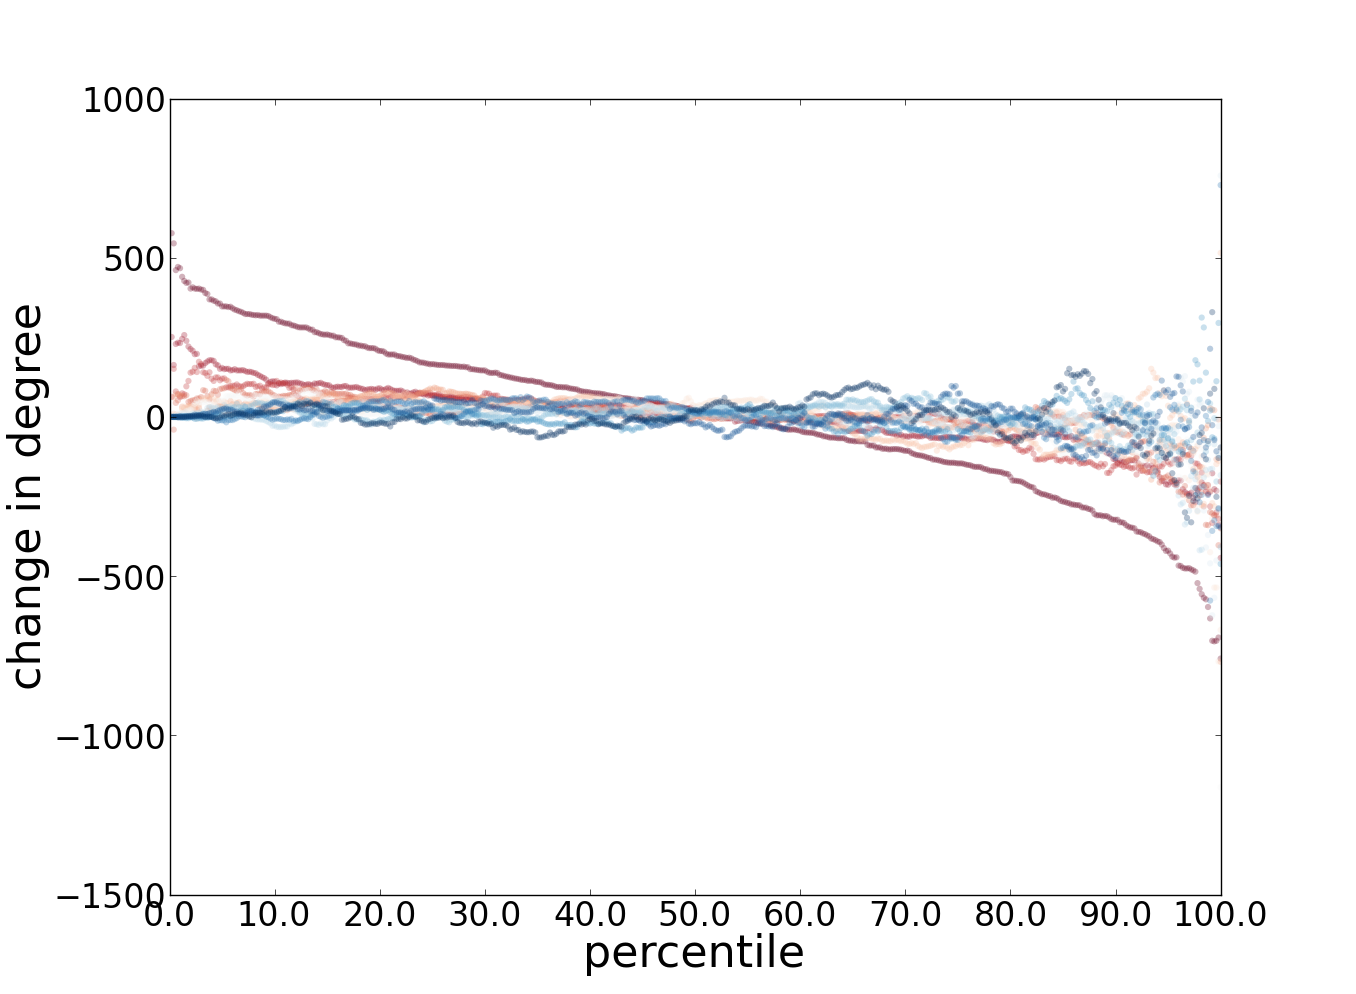
\includegraphics[height=60mm]{n_500_2n3_degchange_percentile}
    \caption{$n^{2}$ timescale}
    \label{fig:100s3}
  \end{subfigure}%
  \caption{Change in degree distribution between each step plotted against percentiles. ($n=500$, $m=250000$)}
\end{figure}

\begin{figure}[h!]
  \vspace{-5mm}
  \begin{subfigure}{0.5\textwidth}
    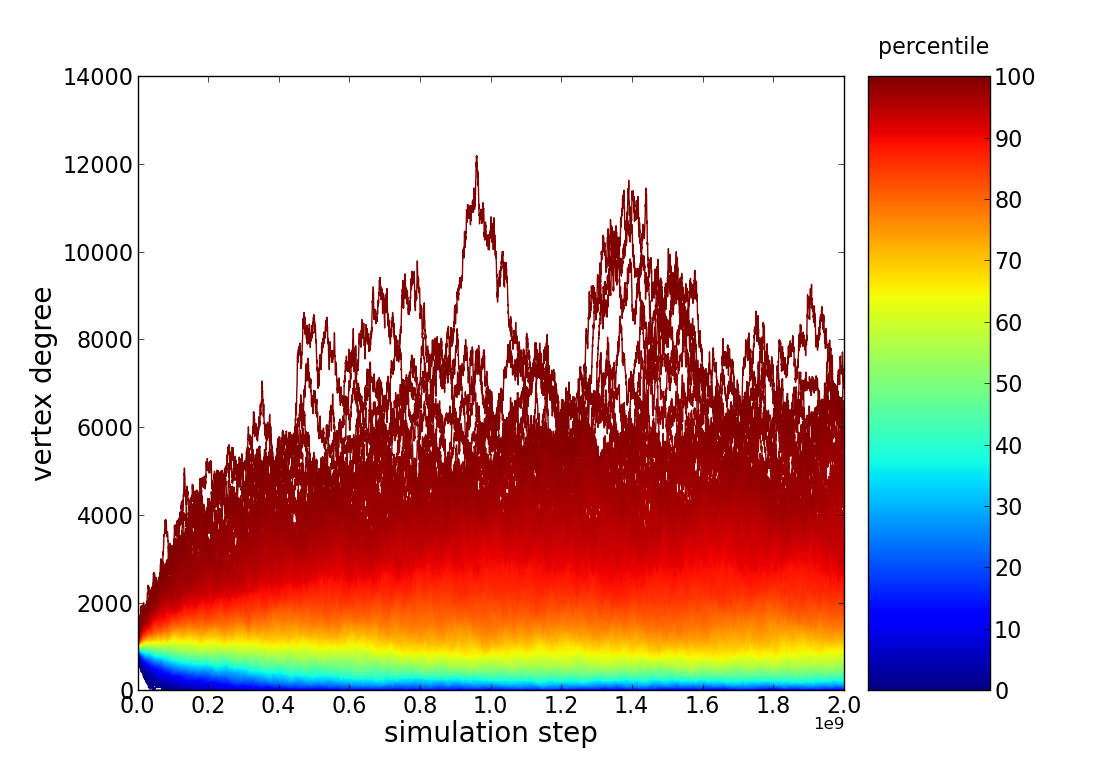
\includegraphics[height=50mm]{n_500_n3_deg_step}
    \caption{$n^{3}$ timescale}
    \label{fig:100s3}
  \end{subfigure}%
  \begin{subfigure}{0.5\textwidth}
    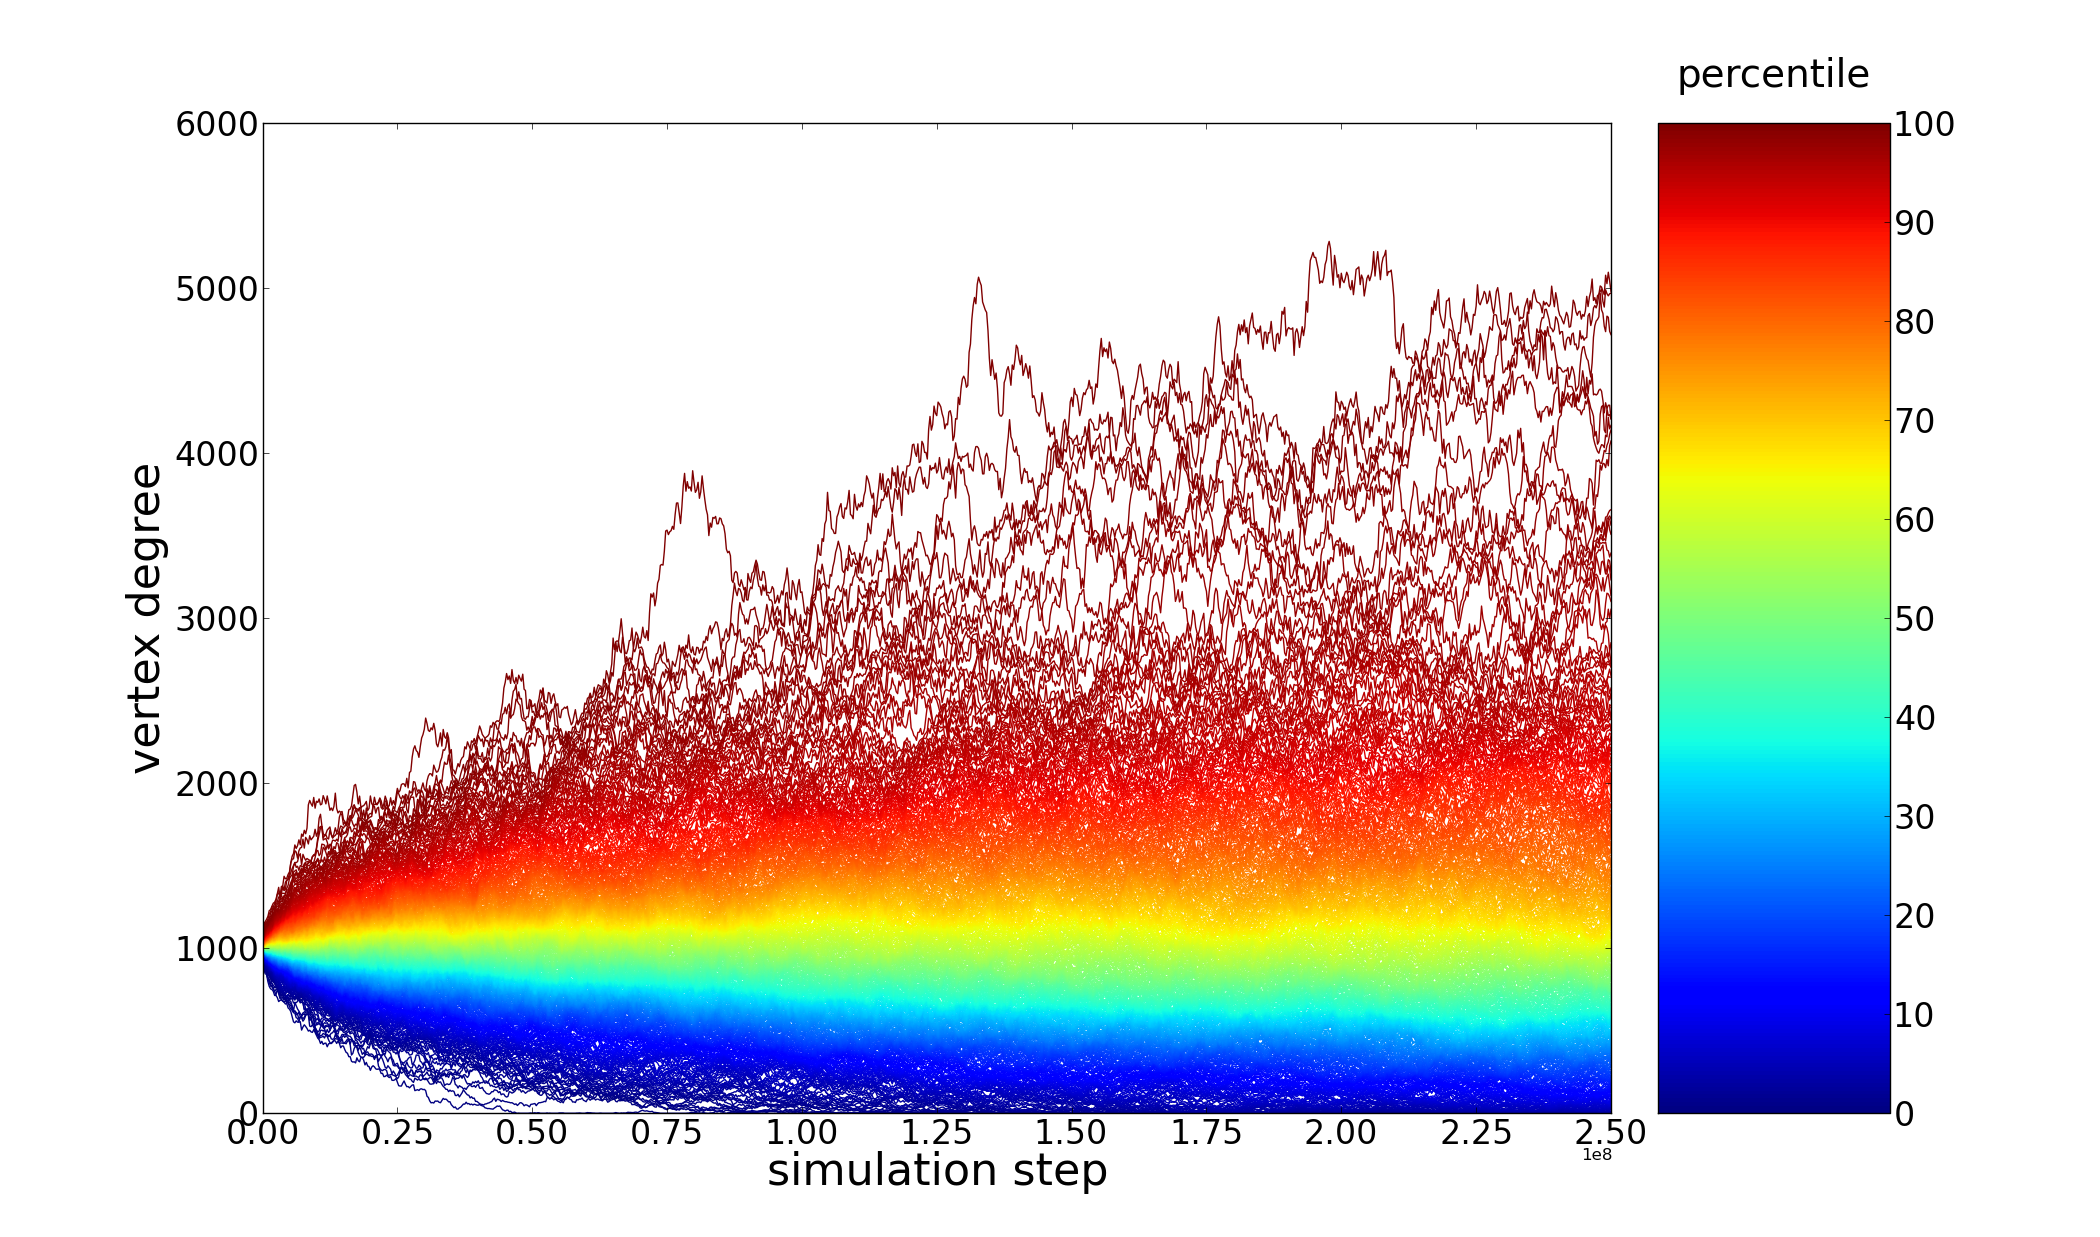
\includegraphics[height=50mm]{n_500_2n3_deg_step}
    \caption{$n^{2}$ timescale}
    \label{fig:100s3}
  \end{subfigure}%
  \caption{Evolution of degree distribution. Color indicates percentile, i.e. the median degree at each step is colored green. ($n=500$, $m=250000$)}
\end{figure}

%% \begin{figure}[h!]
%%   \centering
%%   \includegraphics[height=60mm]{n_500_short}
%%   \caption{$n^{2}$ timescale, $n=500$, $m=250000$}
%%   \label{fig:500sv}
%% \end{figure}
%% \begin{figure}[h!]
%%   \centering
%%   \includegraphics[height=60mm]{n_500_long_3d}
%%   \caption{$n^{3}$ timescale, $n=500$, $m=250000$}
%%   \label{fig:500l3}
%% \end{figure}
%% \begin{figure}[h!]
%%   \centering
%%   \includegraphics[height=60mm]{n_500_long_time}
%%   \caption{$n^{3}$ timescale, $n=500$, $m=250000$}
%%   \label{fig:500lt}
%% \end{figure}
%% \begin{figure}[h!]
%%   \centering
%%   \includegraphics[height=60mm]{n_500_long}
%%   \caption{$n^{3}$ timescale, $n=500$, $m=250000$}
%%   \label{fig:500lv}
%% \end{figure}

%% \begin{figure}[h!]
%%   \centering
%%   \includegraphics[height=60mm]{n_1000_short_3d}
%%   \caption{$n^{2}$ timescale, $n=1000$, $m=1000000$}
%%   \label{fig:1000s3}
%% \end{figure}
%% \begin{figure}[h!]
%%   \centering
%%   \includegraphics[height=60mm]{n_1000_short_time}
%%   \caption{$n^{2}$ timescale, $n=1000$, $m=1000000$}
%%   \label{fig:1000st}
%% \end{figure}
%% \begin{figure}[h!]
%%   \centering
%%   \includegraphics[height=60mm]{n_1000_short}
%%   \caption{$n^{2}$ timescale, $n=1000$, $m=1000000$}
%%   \label{fig:1000sv}
%% \end{figure}
%% \begin{figure}[h!]
%%   \centering
%%   \includegraphics[height=60mm]{n_1000_long_3d}
%%   \caption{$n^{3}$ timescale, $n=1000$, $m=1000000$}
%%   \label{fig:1000l3}
%% \end{figure}
%% \begin{figure}[h!]
%%   \centering
%%   \includegraphics[height=60mm]{n_1000_long_time}
%%   \caption{$n^{3}$ timescale, $n=1000$, $m=1000000$}
%%   \label{fig:1000lt}
%% \end{figure}
%% \begin{figure}[h!]
%%   \centering
%%   \includegraphics[height=60mm]{n_1000_long}
%%   \caption{$n^{3}$ timescale, $n=1000$, $m=1000000$}
%%   \label{fig:1000lv}
%% \end{figure}


\end{changemargin}

\end{document}
